\documentclass[xcolor=dvipsnames,table]{beamer}
\useinnertheme{rounded}
\useoutertheme{infolines}

\usepackage[portuguese]{babel}
\usepackage[utf8]{inputenc}
\usepackage{url}
\usepackage{multicol}

\title{Aplicação cliente-servidor baseada em KVS com TLS}
\subtitle{Tópicos em Redes de Computadores (INFO-7065)}
\author{Josiney de Souza (josiney.souza@ifc.edu.br)}
\institute{UFPR / DInf}
\date{\today}

%%% Apagar barra de navegacao:
% https://stackoverflow.com/questions/3210205/how-to-get-rid-of-navigation-bars-in-beamer
% https://stackoverflow.com/questions/1435837/how-to-remove-footers-of-latex-beamer-templates
\beamertemplatenavigationsymbolsempty
%%% Remover o titulo, autor e data do rodape:
% https://tex.stackexchange.com/questions/113443/remove-author-and-institution-in-footline
\beamertemplatefootempty

%%% Cores das fontes:
% https://en.wikibooks.org/wiki/LaTeX/Colors
\definecolor{ifvermelho}{RGB}{200,12,15}
\definecolor{ifverde}{HTML}{2F9E41}
% Mais cores feitas com http://coolors.co
\definecolor{ifvermelho2}{HTML}{B60B0E} % Nome: International Orange Engineering
\definecolor{ifvermelho3}{HTML}{A50A0D} % Nome: Rufous
\definecolor{ifmeioesq}{HTML}{A2311C} % Nome: Chinese Red
\definecolor{ifmeio}{HTML}{7C5528} % Nome: Coyote Brown
\definecolor{ifmeiodir}{HTML}{567A35} % Nome: Sap Green
\definecolor{ifverde2}{HTML}{42A752} % Nome: Green Pigment
\definecolor{ifverde3}{HTML}{53AF62} % Nome: Medium Sea Green

% https://tex.stackexchange.com/questions/133820/beamer-how-to-change-color-of-infolines-and-frame-title
\setbeamercolor{title}{fg=Red}
\setbeamercolor{frametitle}{fg=Red}
\setbeamercolor{section in head/foot}{fg=White,bg=ifvermelho}
\setbeamercolor{subsection in head/foot}{fg=ifverde}

%%% Cores das caixas de block, exemplo e alerta
% https://tex.stackexchange.com/questions/33231/how-to-change-the-color-of-a-block-within-a-custom-beamer-sty-theme-file
\setbeamercolor{block title}{fg=White,bg=ifverde2}
\setbeamercolor{block body}{fg=White,bg=ifverde3}
% https://tex.stackexchange.com/questions/73163/change-color-scheme-for-example-box-in-beamer
\setbeamercolor{block title example}{fg=White,bg=ifmeio}
\setbeamercolor{block body example}{fg=White,bg=ifmeiodir}
% https://tex.stackexchange.com/questions/96686/change-color-of-itemize-in-beamer-alertblock
\setbeamercolor{block title alerted}{fg=White,bg=ifvermelho3}
\setbeamercolor{block body alerted}{fg=White,bg=ifvermelho2}

%%% Mostrar o sumario novamente antes do inicio da proxima secao
% https://pt.overleaf.com/learn/latex/beamer
\AtBeginSection[]
{\small
  \begin{frame}[plain]
    \frametitle{Sumário}
    \tableofcontents[currentsection]
%	\begin{multicols}{2}
%	\tableofcontents[currentsection]
%	\end{multicols}
  \end{frame}
}

%%% Plano de fundo usado no modelo ODT/DOC/DOCX da Cecom
\usebackgroundtemplate%
{%
    
\includegraphics[width=\paperwidth,height=\paperheight]{fundo.jpg}%
}



%%%%%%%%%%%%%%%%%%%%%%%%%%%%%%%%%%%%%%%%%%%%%%%%%%%
%%%%%%%%%%%%%%% Início do documento %%%%%%%%%%%%%%%
%%%%%%%%%%%%%%%%%%%%%%%%%%%%%%%%%%%%%%%%%%%%%%%%%%%
\begin{document}

%%%%% Primeira página do modelo abaixo - PODE SER REMOVIDA, SE DESEJAR %%%%%
%%% Centralizando o titulo da primeira pagina
% https://stackoverflow.com/questions/2365539/centering-titles-when-using-the-beamer-class-in-latex
%%% Removendo as formatacoes do slide
% https://tex.stackexchange.com/questions/281334/left-aligned-title-page-in-beamer-boadilla-usetheme
%{
%\usebackgroundtemplate%
%{%
%    
\includegraphics[width=\paperwidth,height=\paperheight]{primeira-pag-menor.jpg}%
%}
%\begin{frame}[plain]{\centerline{\inserttitle}}
%\end{frame}
%}
%%%%% Primeira página do modelo acima - PODE SER REMOVIDA, SE DESEJAR %%%%%

\begin{frame}[plain]{}
    \maketitle
\end{frame}

{\small
\begin{frame}[plain]{Sumário}
    \tableofcontents
%	\begin{multicols}{2}
%	\tableofcontents
%	\end{multicols}
\end{frame}
}

%%%%%%%%%%%%%%%%%%%%%%%%%%%%%%%%%%%%%%%%%%%%%%%%%%%%%%%%%%%%%%%%%%%%%
\section{Introdução}
\subsection{A especificação do trabalho}
\begin{frame}{A especificação do trabalho}
	Esta é a segunda avaliação de 2023/1 de Tópicos em Redes de Computadores:
	\begin{itemize}
		\item Fazer uma aplicação cliente/servidor
		\item Baseada em KVS (Key-Value Store)
		\item Usar TLS (Transport Layer Security)
		\item Demonstrar SIGILO
		\item Demonstrar AUTENTICIDADE
		\item Demonstrar INTEGRIDADE
	\end{itemize}
	Página do componente curricular (disciplina/matéria): \url{https://www.inf.ufpr.br/elias/topredes/}
\end{frame}

\begin{frame}{Entrega}
	O formato de entrega do trabalho:
	\begin{description}
		\item[Relatório:] pode ser vídeo, apresentação ou relatório em texto;
		\begin{itemize}
			\item Optei por este vídeo
		\end{itemize} \pause
		
		\item[\textit{Logs} de execução:] via demonstrações no vídeo ou \textit{logs} em uma página \textit{web};
		\begin{itemize}
			\item Optei por ambos
			\item Página: \url{https://www.inf.ufpr.br/jsouza/}
		\end{itemize} \pause
		
		\item[Código comentado:] entrega do código comentado
		\begin{itemize}
			\item Página: \url{https://www.inf.ufpr.br/jsouza/}
			\item GitHub: \url{https://github.com/josiney-souza/ufpr-topicos-redes}
		\end{itemize}
	\end{description}
	Entrega por e-mail
\end{frame}

\subsection{A organização do sistema/aplicação}
\begin{frame}{A organização do sistema/aplicação}
	O sistema está assim organizado - \textbf{códigos}:
	\begin{description}
		\item[Linguagem:] Python
		\item[02-cliente.py:] aplicação cliente - entra em contato com o servidor para solicitar serviços ou recursos;
		\item[02-servidor.py:] aplicação servidor - recebe as demandas dos clientes e retorna alguma ação;
		\item[02-invasor.py:] aplicação cliente não autorizada a se comunicar com o servidor;
		\item[confs\_comuns.py:] biblioteca pessoal de funções e configurações comuns aos clientes e ao servidor.
	\end{description}
\end{frame}

\begin{frame}{A organização do sistema/aplicação}
	O sistema está assim organizado - \textbf{outros arquivos}:
	\begin{description}
		\item[id\_dsa.pub:] chave \underline{pública} criada com \texttt{ssh-keygen(1)}
		\item[id\_dsa:] chave \underline{privada} criada com \texttt{ssh-keygen(1)}
		\begin{itemize}
			\item \texttt{\$ ssh-keygen}
		\end{itemize} \pause
		
		\item[cert-rsa.pem:] certificado auto-assinado para uso no servidor
		\begin{itemize}
			\item \texttt{\$ openssl req -newkey rsa:2048 -nodes -keyout id\_dsa -x509 -days 365 -out cert-rsa.pem}
		\end{itemize}
	\end{description}
\end{frame}

%\begin{frame}{}
%	T
%\end{frame}

\section{Demonstrando uso normal}
\begin{frame}{Uso normal}
	O funcionamento normal envolve um menu:
	\begin{description}
		\item[1:] Adicionar uma chave e um valor;
		\item[2:] Consultar uma chave;
		\item[3:] Consultar todo o banco;
		\item[4:] Atualizar um valor a partir de uma chave;
		\item[5:] Apagar uma chave e um valor;
		\item[6:] Apagar toda a base; \pause
		\item[7:] Demonstrar INTEGRIDADE; \pause
		\item[?:] Mostrar o menu de ajuda\footnote{na verdade, qualquer opção não reconhecida. Caso padrão};
		\item[ad:] \underline{\textbf{A}}tivar a \underline{\textbf{D}}epuração/\textit{Debug};
		\item[dd:] \underline{\textbf{D}}ESativar a \underline{\textbf{D}}epuração/\textit{Debug};
		\item[0:] Encerrar a conexão e sair.
	\end{description}
\end{frame}

\section{Demonstrando SIGILO}
\begin{frame}{Demonstrando SIGILO}
	Para demonstrar que o sistema cliente/servidor possui a característica de \underline{SIGILO} do TLS:
	\begin{enumerate}
		\item Iniciar o Wireshark;
		\begin{itemize}
			\item \texttt{\$ sudo wireshark}
		\end{itemize}
		\item Capturar os pacotes TCP relacionados à porta 8003
		\begin{itemize}
			\item regra \texttt{tcp.port > 8000}\footnote{É de mais de 8.000!!! \url{https://www.youtube.com/watch?v=S8IL1JJuJiE}}
		\end{itemize}
		\item Iniciar o servidor;
		\begin{itemize}
			\item \texttt{\$ python3 02-servidor.py}
		\end{itemize}
		\item Iniciar o cliente.
		\begin{itemize}
			\item \texttt{\$ python3 02-cliente.py}
		\end{itemize}
	\end{enumerate}
\end{frame}

\section{Demonstrando AUTENTICIDADE}
\begin{frame}{Demonstrando AUTENTICIDADE}
	Para demonstrar a \underline{AUTENTICIDADE} com o uso do TLS no sistema cliente/servidor:
	\begin{enumerate}
		\item Iniciar o servidor;
		\begin{itemize}
			\item \texttt{\$ python3 02-servidor.py}
		\end{itemize}
		\item Iniciar o \textbf{invasor}.
		\begin{itemize}
			\item Sem carregar certificados
			\item \texttt{\$ python3 02-invasor.py} \pause
			\item Carregando certificado errado
			\item \texttt{\$ python3 02-invasor.py}
		\end{itemize}
	\end{enumerate}
\end{frame}

\section{Demonstrando INTEGRIDADE}
\begin{frame}{Demonstrando INTEGRIDADE}
	\begin{enumerate}
		\item Iniciar o servidor;
		\begin{itemize}
			\item \texttt{\$ python3 02-servidor.py}
		\end{itemize}
		\item Iniciar o cliente;
		\begin{itemize}
			\item \texttt{\$ python3 02-cliente.py}
		\end{itemize}
		\item Escolher a opção 7 do menu de interação.
	\end{enumerate}
\end{frame}

\begin{frame}{Demonstrando INTEGRIDADE}
	\begin{enumerate}
		\item[0.1] Cliente solicita serviço (aqui: todo o banco)
		\item[0.2] Simula captura de mensagem criptografada no cliente
		\begin{itemize}
			\item Cifra de Cesar
			\item Chave assimétrica (chave pública cliente - 401)
			\item Cifra de Cesar
		\end{itemize}
	\end{enumerate}
\end{frame}

\subsection{Cifra de Cesar e ROT13}
\begin{frame}{Demonstrando INTEGRIDADE: Cifra de Cesar}
	Cifra de substituição:
	\begin{itemize}
		\item Texto normal: ABCDEFGHIJKLMNOPQRSTUVWXYZ
		\item Texto cifrado: DEFGHIJKLMNOPQRSTUVWXYZABC
		\item Chave: 3
	\end{itemize}
	\begin{center}
		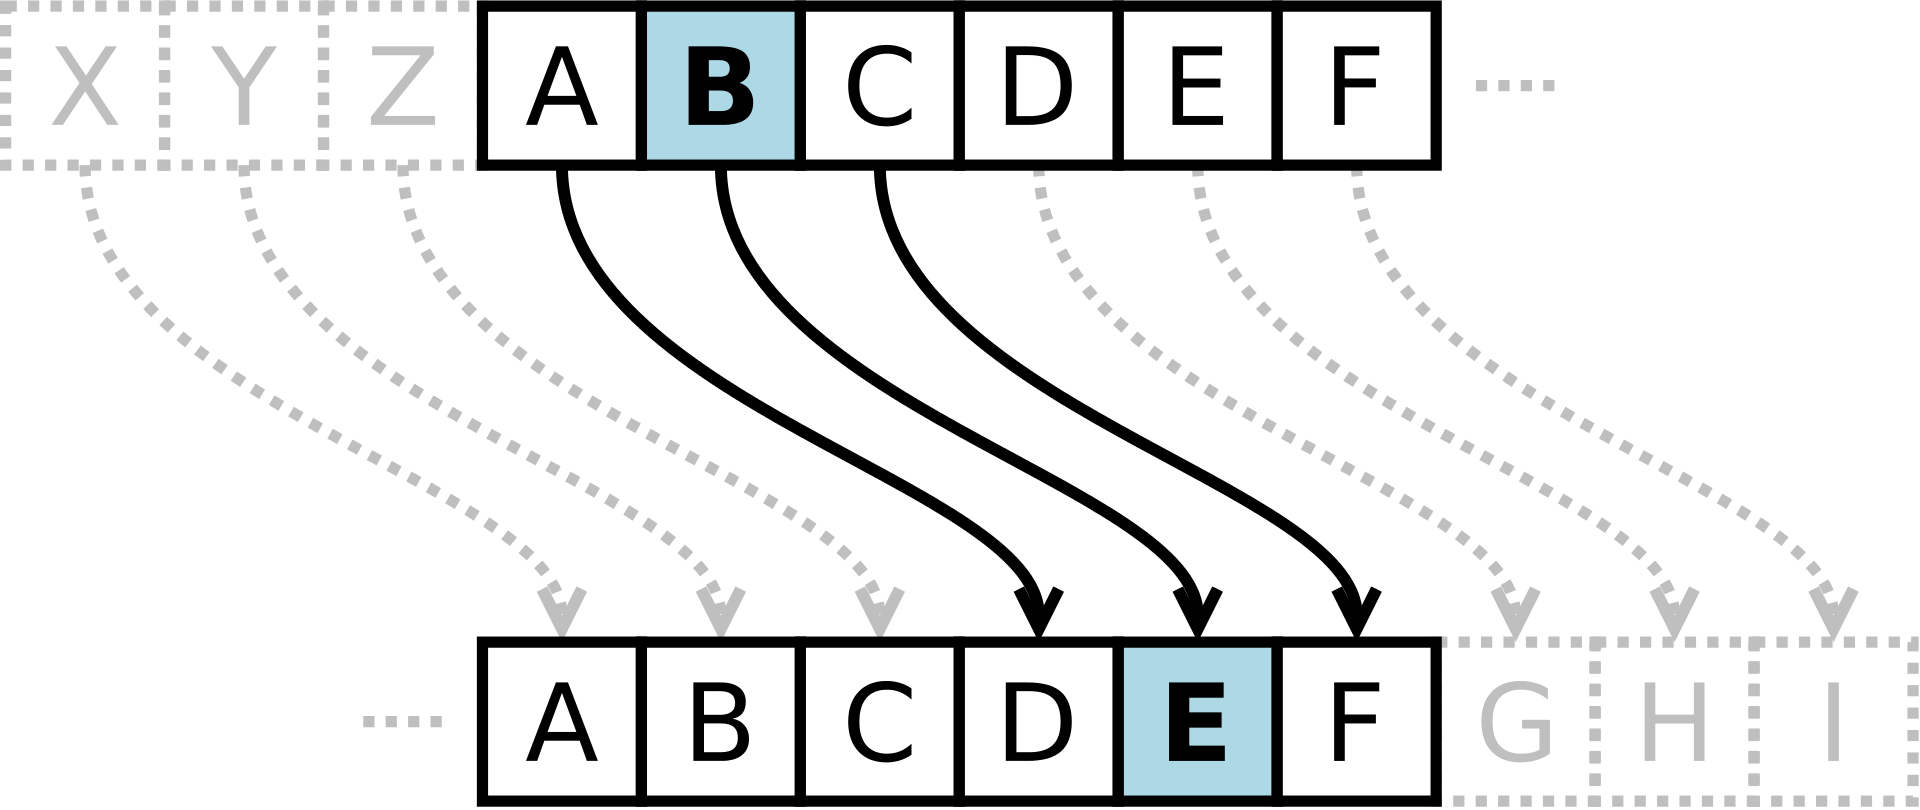
\includegraphics[scale=0.1]{cifra-cesar.png}
	\end{center}
	Fonte: \url{https://pt.wikipedia.org/wiki/Cifra_de_C\%C3\%A9sar\#/media/Ficheiro:Caesar3.svg}
\end{frame}

\begin{frame}{Demonstrando INTEGRIDADE: Cifra de Cesar}
	Cifra de Cesar com rotação 13 (ROT13):
	\begin{center}
		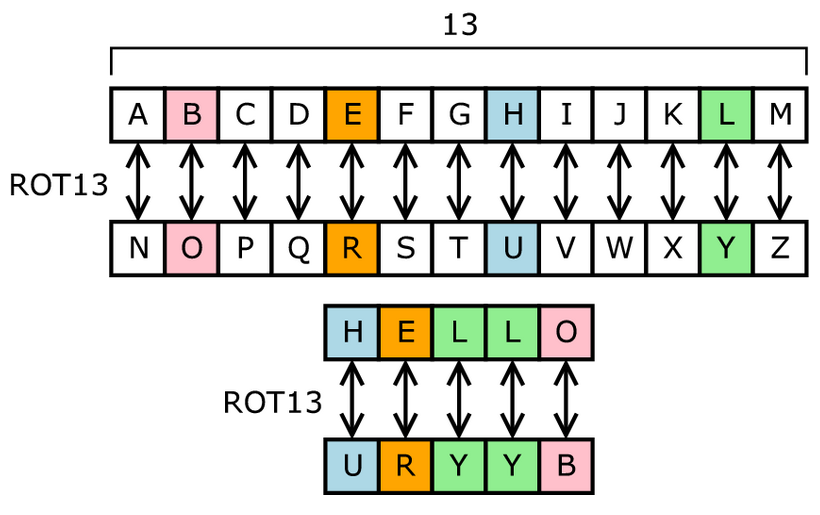
\includegraphics[scale=0.3]{ROT13.png}
	\end{center}
	Fonte: \url{https://pt.wikipedia.org/wiki/ROT13\#/media/Ficheiro:ROT13.png}
\end{frame}

\begin{frame}[fragile]{Demonstrando INTEGRIDADE: Cifra de Cesar}
	Cifra de Cesar em Python - codificando:
	\begin{verbatim}
import codecs
print(codecs.encode("Olá, você!", "rot_13"))
	\end{verbatim}
	\begin{itemize}
		\item ``Olá, você!'' $\rightarrow$ ``Byá, ibpê!''
		\item ``Ççsenha: 123mudar!'' $\rightarrow$ ``Ççfraun: 123zhqne!''
	\end{itemize} \pause
	Cifra de Cesar em Python - \underline{DE}codificando
	\begin{verbatim}
import codecs
print(codecs.decode("Wbfvarl qr Fbhmn", "rot_13"))
	\end{verbatim}
	\begin{itemize}
		\item ``Wbfvarl qr Fbhmn'' $\rightarrow$ ``Josiney de Souza''
	\end{itemize}
\end{frame}

\subsection{Aritmética modular e inverso multiplicativo}
\begin{frame}{Demonstrando INTEGRIDADE: Aritmética modular}
	\begin{itemize}
		\item Aritmética para números inteiros
		\item Números retrocedem quando chega a um máximo
		\item 37 mod 4 = 1
		\begin{description}
			\item[37] dividendo
			\item[4] divisor
			\item[9] quociente
			\item[1] resto
		\end{description}
	\end{itemize} \pause
	Outro exemplo
	\begin{center}
		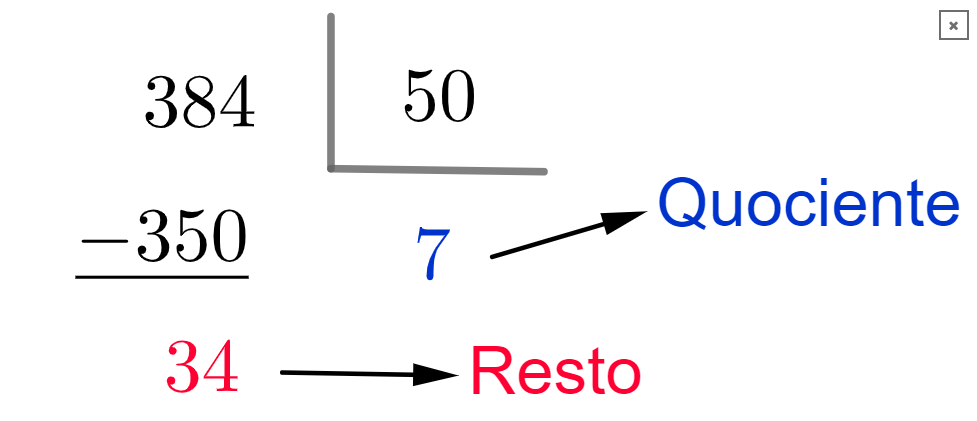
\includegraphics[scale=0.15]{resto-divisao.png}
	\end{center}
	Fonte: \url{https://escolaeducacao.com.br/para-que-serve-o-resto-da-divisao/}
\end{frame}

\begin{frame}[fragile]{Demonstrando INTEGRIDADE: Inverso multiplicativo}
	Descobrir um x e um y tal que x*y mod 1000 = 1
	\begin{itemize}
		\item x * y mod n = 1
		\item 401 * 601 mod 1000 = 1
		\item 191 * 911 mod 1000 = 1
		\item 167 * 503 mod 1000 = 1
	\end{itemize} \pause
	Programa para descobrir o inverso multiplicativo de um número mod 1000:
	\begin{verbatim}
valor = int(input("Que numero quer descobrir o inverso modular
multiplicativo? "))
for i in range(1000):
    if ((valor*i)%1000 == 1):
        print(valor, "x", i, "mod 1000 =", (valor*i)%1000)
	\end{verbatim}
\end{frame}

\begin{frame}{Demonstrando INTEGRIDADE: Inverso multiplicativo}
	Criptografando com uma chave ...
	\begin{itemize}
		\item Caractere 'A' $\rightarrow$ 65 na tabela ASCII
		\item 65 * 191 = 12.415
		\item 12.415 mod 1000 = 415
	\end{itemize} \pause
	Descriptografando com outra chave ...
	\begin{itemize}
		\item Número 415
		\item 415 * 911 = 378.065
		\item 378.065 mod 1000 = 65
		\item Caractere 'A' é recuperado
	\end{itemize}
	Fonte: \url{https://www.inf.ufpr.br/elias/topredes/Sec4TopRedes23.pdf}
\end{frame}

\subsection{Sigilo e Integridade}
\begin{frame}{Demonstrando INTEGRIDADE}
	\begin{enumerate}
		\item[0.1] Cliente solicita serviço (aqui: todo o banco)
		\item[0.2] Simula captura de mensagem criptografada no cliente
		\begin{itemize}
			\item Cifra de Cesar
			\item Chave assimétrica (chave pública cliente - 401)
			\item Cifra de Cesar
		\end{itemize} \pause
		\item simula uma descriptografia com a cifra de Cesar \pause
		\item simula descriptografar usando o inverso multiplicativo da operação de criptografia
		\begin{itemize}
			\item Assume invasor com chave pública 191 $\rightarrow$ ERRO! \pause
			\item Assume cliente com chave pública 401 $\rightarrow$ ERRO! \pause
			\item Assume invasor com chave privada 911 $\rightarrow$ ERRO! \pause
			\item Assume cliente com chave privada 601 $\rightarrow$ OK
		\end{itemize}
		\item simula mais uma descriptografia com a cifra de Cesar
	\end{enumerate}
\end{frame}

\begin{frame}{Demonstrando INTEGRIDADE: Simulando alteração da mensagem}
	\begin{enumerate}
		\item[0.1] Cliente solicita serviço (aqui: todo o banco)
		\item[0.2] Simula captura de mensagem criptografada no cliente
		\begin{itemize}
			\item Cifra de Cesar
			\item Chave assimétrica (chave pública cliente - 401)
			\item Cifra de Cesar
		\end{itemize}
		\item simula alteração de mensagem nos índices 1, 3, 5, 7, 9 \pause
		\item simula uma descriptografia com a cifra de Cesar
		\begin{itemize}
			\item ERRO!
		\end{itemize} \pause
		\item simula descriptografar usando o inverso multiplicativo da operação de criptografia
		\begin{itemize}
			\item Assume cliente com chave privada 601 $\rightarrow$ ``OK''
		\end{itemize}
		\item simula mais uma descriptografia com a cifra de Cesar
	\end{enumerate}
\end{frame}

\begin{frame}[plain]{}
    \maketitle
\end{frame}

%\section{Códifo-fonte}

%%%%% Última página do modelo abaixo - PODE SER REMOVIDA, SE DESEJAR %%%%%
%{
%\usebackgroundtemplate%
%{%
%    
\includegraphics[width=\paperwidth,height=\paperheight]{ultima-pag-menor.jpg}%
%}
%\begin{frame}[plain]{}
%\end{frame}
%}
%%%%% Última página do modelo acima - PODE SER REMOVIDA, SE DESEJAR %%%%%
	
\end{document}